\chapter{Resultados Complementares}
\label{ap:complementares}

Este apêndice reúne as tabelas de detalhe dos resultados do \autoref{cap:resultados}, na ordem das seções daquele capítulo, e as curvas de treino da configuração original (\autoref{subsec:desTreino}).

\section{Linha de Base}

\begin{figure}[H]
    \centering
    \captionsetup{justification=centering}
    \caption{Perda e acurácia por época na configuração original em Indian Pines (semente 42, treino completo)}
    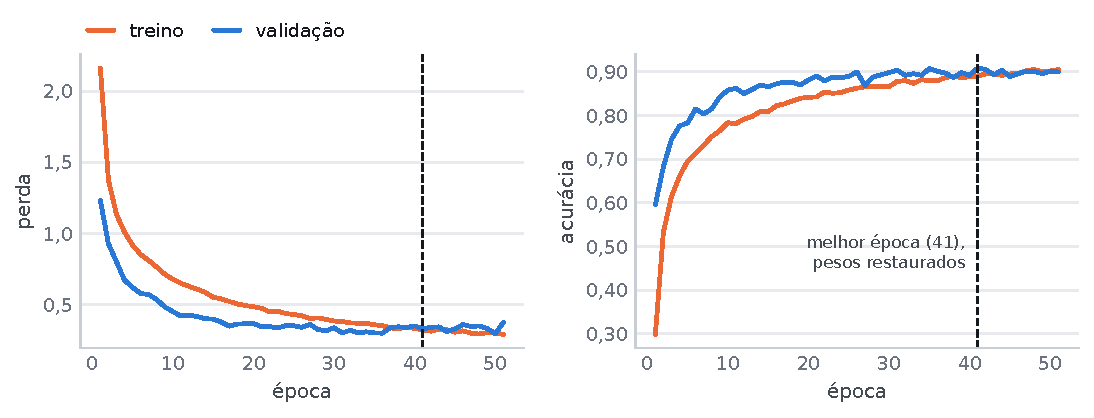
\includegraphics[width=\textwidth]{assets/resultados/curvas_treino.pdf}
    \captionsetup{justification=raggedright}
    \caption*{Fonte: Elaborada pelo autor. A linha tracejada marca a melhor época}
    \label{fig:curvasTreino}
\end{figure}

\begin{table}[H]
    \centering
    \caption{Divisão dos dados e tamanho da rede por cena}
    \footnotesize
    \setlength{\tabcolsep}{4pt}
    \begin{tabular}{|l|c|c|c|C{1.25cm}|c|c|C{1.3cm}|c|}
        \hline
        \rowcolor[HTML]{C0C0C0}
        \textbf{Cena} & \textbf{Rotulados} & \textbf{Classes} & \textbf{Treino} & \textbf{Treino (10\%)} & \textbf{Validação} & \textbf{Teste} & \textbf{Comp. do PCA} & \textbf{Parâmetros} \\
        \hline
        Indian Pines & 10.249 & 16 & 8.711 & 871 & 769 & 769 & 30 & 160.912 \\ \hline
        University of Pavia & 42.776 & 9 & 36.359 & 3.635 & 3.209 & 3.208 & 15 & 37.577 \\ \hline
        Salinas Valley & 54.129 & 16 & 46.009 & 4.602 & 4.060 & 4.060 & 15 & 38.032 \\ \hline
    \end{tabular}
    \captionsetup{justification=raggedright}
    \caption*{Fonte: Elaborada pelo autor. Divisão com a semente 42; o treino de 10\% é sorteado por classe dentro do treino completo}
    \label{tab:dadosCenas}
\end{table}

\begin{table}[H]
    \centering
    \caption{Acurácia por classe em Indian Pines com a configuração original (semente 42, treino completo)}
    \begin{tabular}{|r|l|c|c|c|}
        \hline
        \rowcolor[HTML]{C0C0C0}
        \textbf{Nº} & \textbf{Classe} & \textbf{Pixels} & \textbf{Amostras de teste} & \textbf{Acurácia} \\
        \hline
        1 & \textit{Alfalfa} & 46 & 3 & 0,0000 \\ \hline
        2 & \textit{Corn-notill} & 1.428 & 107 & 0,8692 \\ \hline
        3 & \textit{Corn-mintill} & 830 & 62 & 0,7419 \\ \hline
        4 & \textit{Corn} & 237 & 18 & 0,7778 \\ \hline
        5 & \textit{Grass-pasture} & 483 & 36 & 0,8611 \\ \hline
        6 & \textit{Grass-trees} & 730 & 55 & 1,0000 \\ \hline
        7 & \textit{Grass-pasture-mowed} & 28 & 2 & 1,0000 \\ \hline
        8 & \textit{Hay-windrowed} & 478 & 36 & 1,0000 \\ \hline
        9 & \textit{Oats} & 20 & 2 & 0,5000 \\ \hline
        10 & \textit{Soybean-notill} & 972 & 73 & 0,8767 \\ \hline
        11 & \textit{Soybean-mintill} & 2.455 & 184 & 0,9457 \\ \hline
        12 & \textit{Soybean-clean} & 593 & 44 & 0,8182 \\ \hline
        13 & \textit{Wheat} & 205 & 16 & 1,0000 \\ \hline
        14 & \textit{Woods} & 1.265 & 95 & 1,0000 \\ \hline
        15 & \textit{Buildings-Grass-Trees-Drives} & 386 & 29 & 0,9310 \\ \hline
        16 & \textit{Stone-Steel-Towers} & 93 & 7 & 0,8571 \\ \hline
         & \textbf{Média (AA)} & 10.249 & 769 & 0,8237 \\ \hline
    \end{tabular}
    \captionsetup{justification=raggedright}
    \caption*{Fonte: Elaborada pelo autor. Nomes das classes como distribuídos com a cena}
    \label{tab:porClasse}
\end{table}

\begin{figure}[H]
    \centering
    \captionsetup{justification=centering}
    \caption{Matriz de confusão do teste em Indian Pines, com a configuração original (semente 42)}
    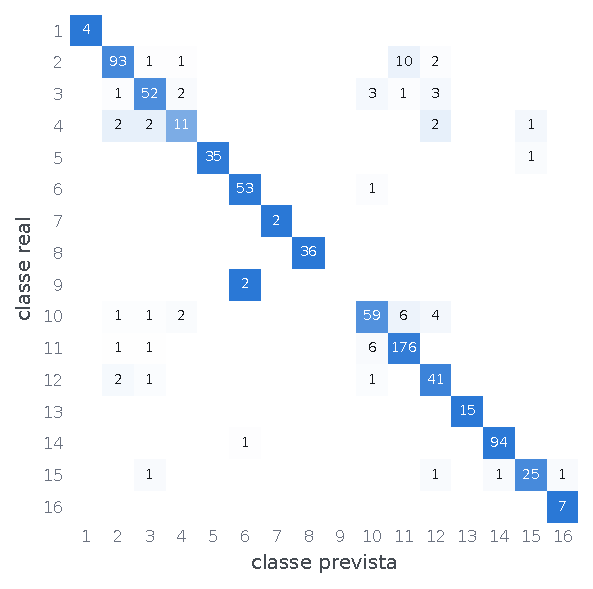
\includegraphics[width=0.72\textwidth]{assets/resultados/matriz_confusao.pdf}
    \captionsetup{justification=raggedright}
    \caption*{Fonte: Elaborada pelo autor. Cada célula traz o número de amostras; a cor, a fração da classe real. Classes numeradas como na \autoref{tab:porClasse}}
    \label{fig:matrizConfusao}
\end{figure}

\section{Organização do Código}

\begin{table}[H]
    \centering
    \caption{Pixels com rótulo diferente entre chamadas do LSC com a mesma imagem e os mesmos parâmetros}
    \begin{tabular}{|l|c|c|c|}
        \hline
        \rowcolor[HTML]{C0C0C0}
        \textbf{Cena} & \textbf{Threads do OpenCV} & \textbf{Pixels diferentes} & \textbf{Fração da cena} \\
        \hline
        Indian Pines & 32 & 401 a 623 & 1,91\% a 2,96\% \\ \hline
         & 1 & 0 & 0 \\ \hline
        University of Pavia & 32 & 222 a 556 & 0,11\% a 0,27\% \\ \hline
         & 1 & 0 & 0 \\ \hline
    \end{tabular}
    \captionsetup{justification=raggedright}
    \caption*{Fonte: Elaborada pelo autor. Catorze chamadas, em duas passadas de 7, comparadas com a primeira chamada de cada passada, com os parâmetros padrão do LSC (\autoref{qua:paramSeg}), na mesma sessão dos tempos da \autoref{tab:estruturaSeg}; a cena tem 21.025 pixels em Indian Pines e 207.400 em University of Pavia}
    \label{tab:lsc}
\end{table}

\begin{table}[H]
    \centering
    \caption{Memória retida por \textit{trial} da busca e projeção para uma campanha de 180 \textit{trials} sem liberação}
    \begin{tabular}{|l|c|c|}
        \hline
        \rowcolor[HTML]{C0C0C0}
        \textbf{Cena} & \textbf{Por \textit{trial} (MB)} & \textbf{180 \textit{trials} retidos (MB)} \\
        \hline
        Indian Pines & 2,5 & 450 \\ \hline
        University of Pavia & 5,1 & 918 \\ \hline
        Salinas Valley & 6,5 & 1.170 \\ \hline
    \end{tabular}
    \captionsetup{justification=raggedright}
    \caption*{Fonte: Elaborada pelo autor. Com a liberação, a memória do processo cresceu 16 MB numa campanha de 180 \textit{trials} em Indian Pines}
    \label{tab:memoria}
\end{table}

\section{Paralelismo}

\begin{table}[H]
    \centering
    \caption{Treino com as threads internas do PyTorch (Indian Pines, 25 épocas, CPU)}
    \begin{tabular}{|c|c|c|}
        \hline
        \rowcolor[HTML]{C0C0C0}
        \textbf{Threads} & \textbf{Tempo (s)} & \textbf{\textit{Speedup} sobre 1 thread} \\
        \hline
        1 & 8,55 & 1,00$\times$ \\ \hline
        2 & 8,45 & 1,01$\times$ \\ \hline
        4 & 7,90 & 1,08$\times$ \\ \hline
        8 & 7,81 & 1,09$\times$ \\ \hline
        16 & 11,67 & 0,73$\times$ \\ \hline
    \end{tabular}
    \captionsetup{justification=raggedright}
    \caption*{Fonte: Elaborada pelo autor. Medição avulsa}
    \label{tab:threadsTorch}
\end{table}

\begin{table}[H]
    \centering
    \caption{Quatro tarefas em sequência e em quatro threads, com e sem o GIL}
    \begin{tabular}{|l|c|c|c|}
        \hline
        \rowcolor[HTML]{C0C0C0}
        \textbf{Tarefa} & \textbf{Sequencial (s)} & \textbf{4 threads (s)} & \textbf{\textit{Speedup}} \\
        \hline
        Laço em Python puro & 1,01 & 0,91 & 1,11$\times$ \\ \hline
        Multiplicação de matrizes (código nativo) & 0,80 & 0,28 & 2,86$\times$ \\ \hline
    \end{tabular}
    \captionsetup{justification=raggedright}
    \caption*{Fonte: Elaborada pelo autor. Medição avulsa}
    \label{tab:gil}
\end{table}

\begin{table}[H]
    \centering
    \caption{Tempo do bloco paralelo da partição da cena, em segundos, e custo de partida dos processos (Indian Pines, modo independente)}
    \small
    \setlength{\tabcolsep}{3pt}
    \begin{tabular}{|c|c|c|C{1.45cm}|C{1.5cm}|c|C{1.5cm}|c|}
        \hline
        \rowcolor[HTML]{C0C0C0}
        \textbf{$N$} & \textbf{Sequencial} & \textbf{Threads} & \textbf{Proc., frio} & \textbf{Proc., quente} & \textbf{Partida} & \textbf{Partida / frio} & \textbf{Aquecimento} \\
        \hline
        2 & 13,58 & 8,45 & 11,08 & 7,31 & 3,77 & 34\% & 3,18 \\ \hline
        4 & 12,96 & 21,39 & 9,12 & 4,51 & 4,61 & 51\% & 3,91 \\ \hline
        8 & 12,29 & 54,14 & 9,01 & 3,34 & 5,67 & 63\% & 4,79 \\ \hline
        16 & 12,81 & 56,59 & 12,95 & 2,86 & 10,09 & 78\% & 7,79 \\ \hline
    \end{tabular}
    \captionsetup{justification=raggedright}
    \caption*{Fonte: Elaborada pelo autor. Médias de 3 repetições com pool quente e 2 com pool frio. Sequencial e threads com pool quente; o \textit{speedup} do pool frio na \autoref{tab:poolQuente} usa a execução sequencial correspondente, de 12,34 s a 13,55 s. Partida: tempo do pool frio menos o do pool quente}
    \label{tab:poolTempos}
\end{table}

\begin{table}[H]
    \centering
    \caption{Acurácia e tempo de uma partição no modo independente (Indian Pines, 25 épocas, lote 64, semente 42)}
    \small
    \setlength{\tabcolsep}{3pt}
    \begin{tabular}{|c|C{1.6cm}|C{1.9cm}|C{2.5cm}|C{1.9cm}|C{2.1cm}|C{1.2cm}|}
        \hline
        \rowcolor[HTML]{C0C0C0}
        \textbf{$N$} & \textbf{Treino por partição} & \textbf{OA, seq. e processos} & \textbf{OA, threads (mín.--máx.)} & \textbf{Partição sozinha (s)} & \textbf{Partição em processos (s)} & \textbf{Razão} \\
        \hline
        2 & 4.355 & 0,9090 & 0,9012--0,9103 & 6,79 & 7,24 & 1,07 \\ \hline
        4 & 2.177 & 0,9155 & 0,9116--0,9207 & 3,24 & 4,45 & 1,37 \\ \hline
        8 & 1.088 & 0,9064 & 0,8999--0,9194 & 1,54 & 3,15 & 2,05 \\ \hline
        16 & 544 & 0,8999 & 0,8921--0,9038 & 0,80 & 2,65 & 3,30 \\ \hline
        32 & 272 & 0,8505 & 0,8296--0,8648 & 0,41 & --- & --- \\ \hline
    \end{tabular}
    \captionsetup{justification=raggedright}
    \caption*{Fonte: Elaborada pelo autor. Treino por partição: média de amostras de treino em cada partição. Partição sozinha: tempo médio de uma partição na execução sequencial; em processos: com as $N$ executando juntas, no pool quente. Com $N$ = 32, só a execução sequencial, porque o pool de processos foi recusado por memória. No modo replicado, a OA foi 0,8830 em todas as execuções}
    \label{tab:particaoOA}
\end{table}

\begin{table}[H]
    \centering
    \caption{Conferência e tempos de referência da fusão concorrente, por cena}
    \small
    \setlength{\tabcolsep}{3pt}
    \begin{tabular}{|l|c|c|C{1.6cm}|C{1.3cm}|C{1.5cm}|C{1.6cm}|C{2.0cm}|}
        \hline
        \rowcolor[HTML]{C0C0C0}
        \textbf{Cena} & \textbf{Posições} & \textbf{Execuções} & \textbf{Ids e classes iguais} & \textbf{OA de teste} & \textbf{Lote, 1 thread (s)} & \textbf{Lote, 16 threads (s)} & \textbf{\mbox{Segmentação} (s)} \\
        \hline
        Indian Pines & 10.249 & 283 & 283 & 0,9051 & 0,330 & 0,196 & 0,111 \\ \hline
        University of Pavia & 42.776 & 220 & 220 & 0,9772 & 1,050 & 0,876 & 0,869 \\ \hline
        Salinas Valley & 54.129 & 220 & 220 & 0,9938 & 1,000 & 0,742 & 0,670 \\ \hline
    \end{tabular}
    \captionsetup{justification=raggedright}
    \caption*{Fonte: Elaborada pelo autor. Execuções: todas as do experimento 14 na cena, incluindo lote e sequencial. Segmentação: ramo espacial executado por T0 (PCA de 3 componentes, composição RGB e SEEDS), média nas execuções sequenciais por blocos}
    \label{tab:fusaoConferencia}
\end{table}

\begin{table}[H]
    \centering
    \caption{Posições cujas convoluções terminaram antes da publicação do mapa, em porcentagem, por número de threads de trabalho}
    \small
    \setlength{\tabcolsep}{3pt}
    \begin{tabular}{|l|l|c|c|c|c|c|c|}
        \hline
        \rowcolor[HTML]{C0C0C0}
        \textbf{Cena} & \textbf{Forma} & \textbf{Bloco} & \textbf{$N$ = 1} & \textbf{$N$ = 2} & \textbf{$N$ = 4} & \textbf{$N$ = 8} & \textbf{$N$ = 16} \\
        \hline
        Indian Pines & como no esquema & 1 & 0,0 & 0,0 & 0,0 & 0,1 & 0,2 \\ \cline{3-8}
         &  & 64 & 0,6 & 1,2 & 2,5 & 5,0 & 10,0 \\ \cline{3-8}
         &  & 1.024 & 10,0 & 20,0 & 40,0 & 79,9 & 100,0 \\ \cline{2-8}
         & desacoplada & 1 & 10,8 & 9,2 & 8,6 & 5,4 & 3,8 \\ \cline{3-8}
         &  & 64 & 94,9 & 100,0 & 100,0 & 100,0 & 100,0 \\ \cline{3-8}
         &  & 1.024 & 94,0 & 100,0 & 100,0 & 100,0 & 100,0 \\ \hline
        University of Pavia & como no esquema & 64 & 0,1 & 0,3 & 0,6 & 1,2 & 2,4 \\ \cline{3-8}
         &  & 1.024 & 2,4 & 4,8 & 9,6 & 19,2 & 38,3 \\ \cline{2-8}
         & desacoplada & 64 e 1.024 & 100,0 & 100,0 & 100,0 & 100,0 & 100,0 \\ \hline
        Salinas Valley & como no esquema & 64 & 0,1 & 0,2 & 0,5 & 0,9 & 1,9 \\ \cline{3-8}
         &  & 1.024 & 1,9 & 3,8 & 7,6 & 15,1 & 30,3 \\ \cline{2-8}
         & desacoplada & 64 e 1.024 & 100,0 & 100,0 & 100,0 & 100,0 & 100,0 \\ \hline
    \end{tabular}
    \captionsetup{justification=raggedright}
    \caption*{Fonte: Elaborada pelo autor. Médias das repetições, com a seção crítica nas duas extensões}
    \label{tab:fusaoSobreposicao}
\end{table}

\begin{table}[H]
    \centering
    \caption{Tempo de parede da fusão concorrente com a seção crítica como no esquema e mínima, em segundos (blocos de 1.024 posições)}
    \footnotesize
    \setlength{\tabcolsep}{3pt}
    \begin{tabular}{|c|c|c|c|c|c|c|}
        \hline
        \rowcolor[HTML]{C0C0C0}
        \multirow{2}{*}{\textbf{$N$}} & \multicolumn{2}{c|}{\textbf{Indian Pines}} & \multicolumn{2}{c|}{\textbf{University of Pavia}} & \multicolumn{2}{c|}{\textbf{Salinas Valley}} \\
        \cline{2-7}
        \rowcolor[HTML]{C0C0C0}
        & \textbf{Esquema} & \textbf{Mínima} & \textbf{Esquema} & \textbf{Mínima} & \textbf{Esquema} & \textbf{Mínima} \\
        \hline
        1 & 0,274 $\pm$ 0,036 & 0,304 $\pm$ 0,064 & 1,006 $\pm$ 0,090 & 1,053 $\pm$ 0,093 & 0,782 $\pm$ 0,024 & 0,869 $\pm$ 0,133 \\ \hline
        2 & 0,201 $\pm$ 0,007 & 0,279 $\pm$ 0,065 & 0,885 $\pm$ 0,054 & 0,905 $\pm$ 0,053 & 0,706 $\pm$ 0,025 & 0,713 $\pm$ 0,049 \\ \hline
        4 & 0,342 $\pm$ 0,016 & 0,363 $\pm$ 0,071 & 0,869 $\pm$ 0,079 & 0,895 $\pm$ 0,068 & 0,705 $\pm$ 0,056 & 0,688 $\pm$ 0,038 \\ \hline
        8 & 0,164 $\pm$ 0,008 & 0,191 $\pm$ 0,036 & 0,948 $\pm$ 0,085 & 0,975 $\pm$ 0,085 & 0,666 $\pm$ 0,014 & 0,687 $\pm$ 0,036 \\ \hline
        16 & 0,171 $\pm$ 0,006 & 0,173 $\pm$ 0,011 & 0,983 $\pm$ 0,086 & 0,986 $\pm$ 0,101 & 0,692 $\pm$ 0,045 & 0,692 $\pm$ 0,047 \\ \hline
    \end{tabular}
    \captionsetup{justification=raggedright}
    \caption*{Fonte: Elaborada pelo autor. Forma como no esquema; média e desvio de 5 repetições}
    \label{tab:fusaoSecao}
\end{table}

\section{Automação de Hiperparâmetros}

\begin{table}[H]
    \centering
    \caption{Diferença entre a melhor e a pior estratégia de busca, por orçamento de épocas (Indian Pines, 3 sementes)}
    \begin{tabular}{|c|l|l|c|c|l|}
        \hline
        \rowcolor[HTML]{C0C0C0}
        \textbf{Orçamento} & \textbf{Melhor} & \textbf{Pior} & \textbf{Diferença (pp)} & \textbf{Desvio comb. (pp)} & \textbf{Leitura} \\
        \hline
        10 épocas & Genética & Aleatória & 1,60 & 2,01 & ruído \\ \hline
        40 épocas & Genética & Aleatória & 2,56 & 1,93 & ruído \\ \hline
        200 épocas & Genética & Aleatória & 2,21 & 3,77 & ruído \\ \hline
    \end{tabular}
    \captionsetup{justification=raggedright}
    \caption*{Fonte: Elaborada pelo autor. Melhor validação de cada busca, média de 3 sementes (\autoref{tab:estrategias}); afirmável quando a diferença excede duas vezes o desvio combinado}
    \label{tab:estrategiasRuido}
\end{table}

\begin{table}[H]
    \centering
    \caption{Como cada estratégia gastou os 20 \textit{trials} (Indian Pines, médias de 3 sementes)}
    \small
    \setlength{\tabcolsep}{3pt}
    \begin{tabular}{|c|l|C{1.8cm}|C{1.8cm}|C{1.8cm}|C{1.8cm}|}
        \hline
        \rowcolor[HTML]{C0C0C0}
        \textbf{Orçamento} & \textbf{Estratégia} & \textbf{\textit{Trial} do melhor} & \textbf{Épocas por \textit{trial}} & \textbf{Treino da busca (s)} & \textbf{\textit{Trials} com SEEDS} \\
        \hline
        10 épocas & Aleatória & 14,0 & 8,7 & 10,1 & 30\% \\
        & TPE & 11,0 & 9,7 & 11,2 & 53\% \\
        & Genética & 13,0 & 9,5 & 10,3 & 55\% \\ \hline
        40 épocas & Aleatória & 6,7 & 36,2 & 38,5 & 30\% \\
        & TPE & 6,7 & 35,8 & 32,4 & 33\% \\
        & Genética & 16,0 & 36,9 & 33,2 & 38\% \\ \hline
        200 épocas & Aleatória & 11,3 & 66,9 & 65,0 & 30\% \\
        & TPE & 18,7 & 67,9 & 64,1 & 33\% \\
        & Genética & 10,7 & 77,8 & 64,7 & 33\% \\ \hline
    \end{tabular}
    \captionsetup{justification=raggedright}
    \caption*{Fonte: Elaborada pelo autor. \textit{Trial} do melhor: posição, entre os 20, do \textit{trial} de maior validação. Épocas por \textit{trial}: épocas efetivamente treinadas, abaixo do teto quando a parada antecipada atua}
    \label{tab:estrategiasCusto}
\end{table}

\begin{table}[H]
    \centering
    \caption{Acurácia de validação média por valor de cada hiperparâmetro (540 \textit{trials} do experimento 08, Indian Pines)}
    \begin{tabular}{|l|l|c|c|c|}
        \hline
        \rowcolor[HTML]{C0C0C0}
        \textbf{Hiperparâmetro} & \textbf{Valor} & \textbf{Validação média} & \textbf{\textit{Trials}} & \textbf{Amplitude (pp)} \\
        \hline
        \multirow{3}{*}{Dropout} & 0,20 & 0,6927 & 220 & \multirow{3}{*}{18,10} \\ \cline{2-4}
         & 0,35 & 0,6368 & 194 &  \\ \cline{2-4}
         & \textbf{0,50} & 0,5117 & 126 &  \\ \hline
        \multirow{3}{*}{Taxa de aprendizado} & 0,0003 & 0,5162 & 120 & \multirow{3}{*}{15,26} \\ \cline{2-4}
         & \textbf{0,001} & 0,6592 & 254 &  \\ \cline{2-4}
         & 0,003 & 0,6688 & 166 &  \\ \hline
        \multirow{4}{*}{Segmentador} & \textbf{SEEDS} & 0,6925 & 202 & \multirow{4}{*}{14,89} \\ \cline{2-4}
         & SLIC & 0,5436 & 90 &  \\ \cline{2-4}
         & LSC & 0,6356 & 148 &  \\ \cline{2-4}
         & Watershed & 0,5752 & 100 &  \\ \hline
        \multirow{3}{*}{Componentes do PCA} & 15 & 0,5750 & 153 & \multirow{3}{*}{8,35} \\ \cline{2-4}
         & \textbf{30} & 0,6585 & 174 &  \\ \cline{2-4}
         & 45 & 0,6472 & 213 &  \\ \hline
        \multirow{3}{*}{\textit{Weight decay}} & \textbf{0} & 0,6497 & 196 & \multirow{3}{*}{4,55} \\ \cline{2-4}
         & $10^{-5}$ & 0,6339 & 176 &  \\ \cline{2-4}
         & $10^{-4}$ & 0,6042 & 168 &  \\ \hline
        \multirow{3}{*}{Tamanho do lote} & \textbf{32} & 0,6186 & 160 & \multirow{3}{*}{1,81} \\ \cline{2-4}
         & 64 & 0,6343 & 221 &  \\ \cline{2-4}
         & 128 & 0,6367 & 159 &  \\ \hline
    \end{tabular}
    \captionsetup{justification=raggedright}
    \caption*{Fonte: Elaborada pelo autor. Em negrito, o valor da configuração original. Amplitude: diferença entre o melhor e o pior valor do hiperparâmetro}
    \label{tab:eixos}
\end{table}

\begin{table}[H]
    \centering
    \caption{Configuração original contra configuração otimizada em AA, Kappa e épocas treinadas (Indian Pines, 5 sementes, 10\% do treino)}
    \small
    \setlength{\tabcolsep}{3pt}
    \begin{tabular}{|l|l|c|c|C{1.3cm}|C{1.3cm}|l|}
        \hline
        \rowcolor[HTML]{C0C0C0}
        \textbf{Segmentador} & \textbf{Métrica} & \textbf{Original} & \textbf{Otimizada} & \textbf{Ganho (pp)} & \textbf{Limiar (pp)} & \textbf{Leitura} \\
        \hline
        \multirow{3}{*}{SEEDS} & AA & 0,5903 $\pm$ 0,0307 & 0,6985 $\pm$ 0,0443 & +10,81 & 10,78 & afirmável \\ \cline{2-7}
         & Kappa & 0,7058 $\pm$ 0,0203 & 0,7910 $\pm$ 0,0131 & +8,52 & 4,83 & afirmável \\ \cline{2-7}
         & Épocas & 53,0 & 80,4 &  &  &  \\ \hline
        \multirow{3}{*}{SLIC} & AA & 0,4071 $\pm$ 0,1550 & 0,4835 $\pm$ 0,1707 & +7,64 & 46,12 & ruído \\ \cline{2-7}
         & Kappa & 0,5342 $\pm$ 0,2087 & 0,5839 $\pm$ 0,2211 & +4,97 & 60,81 & ruído \\ \cline{2-7}
         & Épocas & 71,0 & 115,4 &  &  &  \\ \hline
        \multirow{3}{*}{LSC} & AA & 0,4343 $\pm$ 0,0501 & 0,6104 $\pm$ 0,0298 & +17,61 & 11,67 & afirmável \\ \cline{2-7}
         & Kappa & 0,6294 $\pm$ 0,0469 & 0,7310 $\pm$ 0,0256 & +10,16 & 10,69 & ruído \\ \cline{2-7}
         & Épocas & 73,0 & 64,6 &  &  &  \\ \hline
        \multirow{3}{*}{Watershed} & AA & 0,3847 $\pm$ 0,1534 & 0,4224 $\pm$ 0,2582 & +3,77 & 60,07 & ruído \\ \cline{2-7}
         & Kappa & 0,5056 $\pm$ 0,2118 & 0,4777 $\pm$ 0,2847 & $-$2,79 & 70,98 & ruído \\ \cline{2-7}
         & Épocas & 82,2 & 72,4 &  &  &  \\ \hline
    \end{tabular}
    \captionsetup{justification=raggedright}
    \caption*{Fonte: Elaborada pelo autor. Limiar: duas vezes o desvio combinado das duas configurações. Épocas: média das épocas treinadas até a parada}
    \label{tab:impactoHPOCompleto}
\end{table}

\section{Segmentadores}

\begin{table}[H]
    \centering
    \caption{AA, Kappa e diferença de OA para o SEEDS sob otimização conjunta (5 sementes, 10\% do treino)}
    \footnotesize
    \setlength{\tabcolsep}{3pt}
    \begin{tabular}{|l|l|c|c|C{1.4cm}|C{1.2cm}|l|}
        \hline
        \rowcolor[HTML]{C0C0C0}
        \textbf{Cena} & \textbf{Segmentador} & \textbf{AA} & \textbf{Kappa} & \textbf{Dif. de OA (pp)} & \textbf{Limiar (pp)} & \textbf{Leitura} \\
        \hline
        \multirow{4}{*}{Indian Pines} & SEEDS & 0,6985 $\pm$ 0,0443 & 0,7910 $\pm$ 0,0131 & --- & --- & referência \\ \cline{2-7}
         & SLIC & 0,4835 $\pm$ 0,1707 & 0,5839 $\pm$ 0,2211 & $-$17,63 & 37,19 & ruído \\ \cline{2-7}
         & LSC & 0,6104 $\pm$ 0,0298 & 0,7310 $\pm$ 0,0256 & $-$5,18 & 4,95 & afirmável \\ \cline{2-7}
         & Watershed & 0,4224 $\pm$ 0,2582 & 0,4777 $\pm$ 0,2847 & $-$25,28 & 45,15 & ruído \\ \hline
        \multirow{4}{*}{University of Pavia} & SEEDS & 0,9323 $\pm$ 0,0116 & 0,9358 $\pm$ 0,0055 & --- & --- & referência \\ \cline{2-7}
         & SLIC & 0,9249 $\pm$ 0,0092 & 0,9381 $\pm$ 0,0051 & +0,19 & 1,14 & ruído \\ \cline{2-7}
         & LSC & 0,7422 $\pm$ 0,3156 & 0,7283 $\pm$ 0,3642 & $-$11,82 & 39,73 & ruído \\ \cline{2-7}
         & Watershed & 0,9394 $\pm$ 0,0122 & 0,9410 $\pm$ 0,0026 & +0,41 & 0,93 & ruído \\ \hline
        \multirow{4}{*}{Salinas Valley} & SEEDS & 0,9497 $\pm$ 0,0155 & 0,9590 $\pm$ 0,0084 & --- & --- & referência \\ \cline{2-7}
         & SLIC & 0,9122 $\pm$ 0,0060 & 0,9445 $\pm$ 0,0050 & $-$1,31 & 1,76 & ruído \\ \cline{2-7}
         & LSC & 0,9493 $\pm$ 0,0098 & 0,9453 $\pm$ 0,0060 & $-$1,23 & 1,86 & ruído \\ \cline{2-7}
         & Watershed & 0,9321 $\pm$ 0,0183 & 0,9440 $\pm$ 0,0052 & $-$1,35 & 1,77 & ruído \\ \hline
    \end{tabular}
    \captionsetup{justification=raggedright}
    \caption*{Fonte: Elaborada pelo autor. Limiar: duas vezes o desvio combinado do segmentador e do SEEDS. Em University of Pavia, o LSC colapsou em uma das cinco sementes}
    \label{tab:segmentadoresCompleto}
\end{table}
